\subsection{Final model} \label{subsec:finalmodel}

After training multiple models with different configurations of parameters we have selected the final model. During the process of selection, we have applied the parameters that have worked the best on the baseline model and combined them in various ways. We also adjusted some parameters again to find the best-performing model. Overall we have trained more than 200 models, which took more than 800 hours. 

The final model has the following settings of parameters: 

\begin{itemize}
    \setlength\itemsep{1px}
    \item activation function Leaky RELU with a slope of 0.05 
    \item batch size of 64
    \item optimizer ADAM with betas = 0.9, 0.999
    \item starting learning rate of $1e^{-3}$ 
    \item ReduceLROnplateau scheduler with a decreasing factor = 0.9, threshold = $1e^{-2}$ and patience = 2
    \item dropout in fully-connected layer with probability = 0.5
    \item L2 regularization with $\lambda$ set to $1e^{-5}$
\end{itemize}

On the validation set, it achieved 81.00 \% accuracy on the real data and 99.41 \% on the synthetic data. The evolution of loss and accuracy during training is illustrated in the Figure \ref{fig:lossaccm22}. 

\begin{figure}[!h]
\centering
    \begin{subfigure}[t]{.45\textwidth}
        \centering
        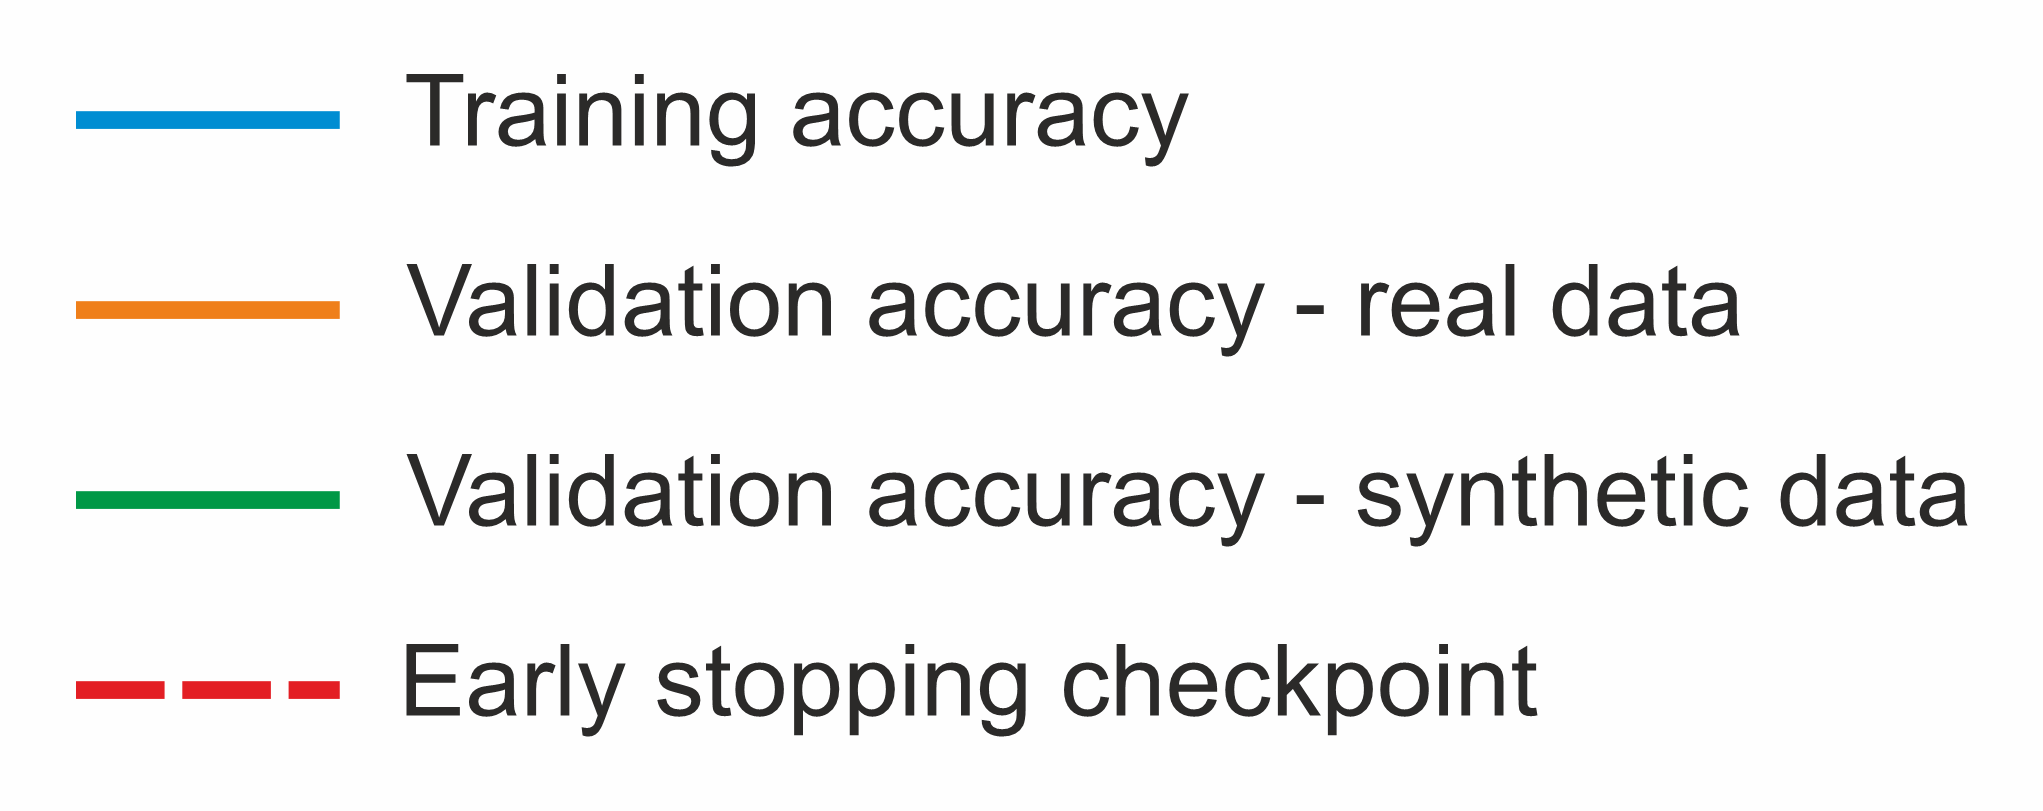
\includegraphics[width=.7\textwidth]{images/popisAc.png}
        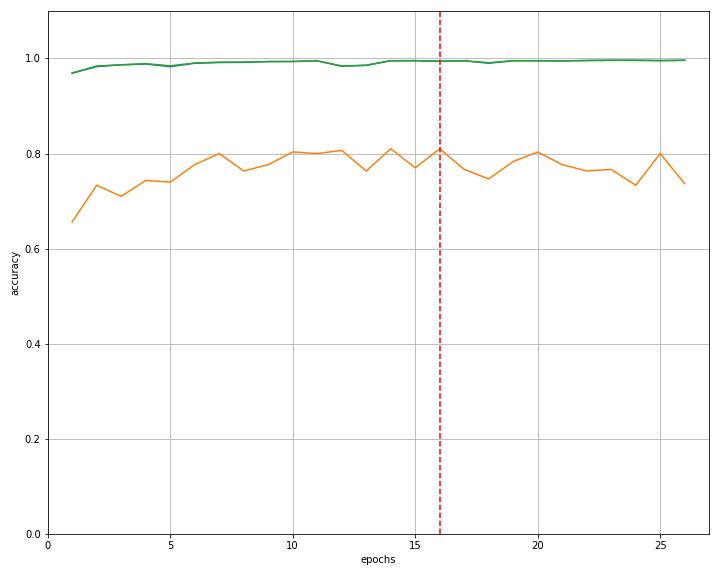
\includegraphics[width=\textwidth]{images/accuracy51ss2_0.png}
        \caption{The accuracy during training.}
        \label{fig:accm22}
    \end{subfigure}
    \begin{subfigure}[t]{.45\textwidth}
        \centering
        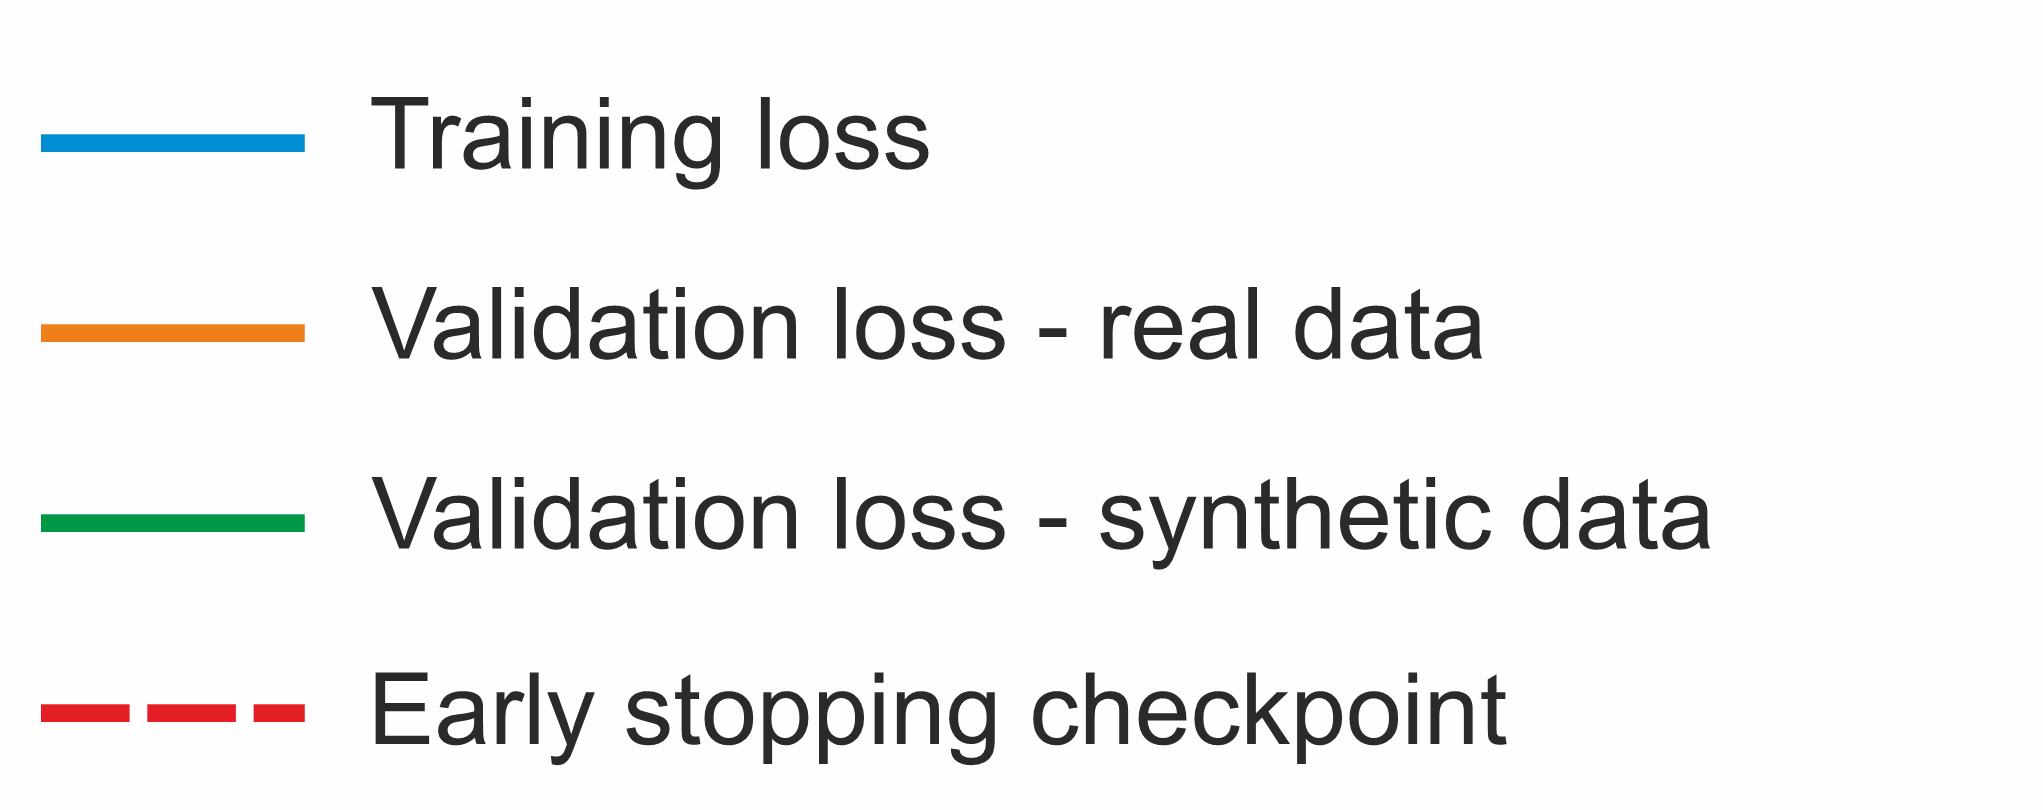
\includegraphics[width=.7\textwidth]{images/popisLoss.png}
        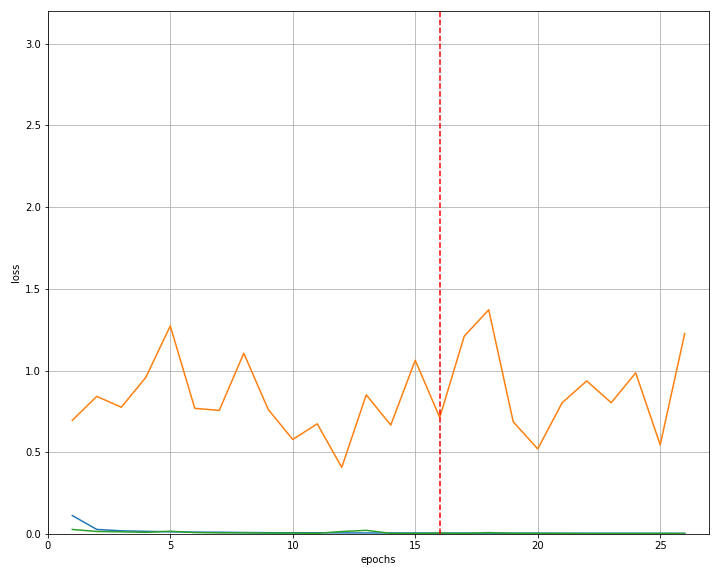
\includegraphics[width=\textwidth]{images/losses51ss2_0.png}
        \caption{The loss during training.}
        \label{fig:lossm22}
    \end{subfigure}

    \caption{The evolution of the loss and accuracy during training of the final model on the synthetic data.}
    \label{fig:lossaccm22}
\end{figure}

